\chapter{Background}
etwas mehr als man braucht um die arbeit zu verstehen. Aber nicht viel mehr.
To me before I wrote this:
\subsection{Stencil computation}
Stencil codes can be categorized by various properties like the dimensionality of the grid, the locality of the stencil, the boundary condition or the shape.
The focus of this work lies on linear, two dimensional star-shaped stencils, meaning that the underlying grid is two dimensional, each cell is only updated by neighbors along the axes and no diagonals and the the new value of a cell is a linear function of the neighbors values.
The category of stencils that also involve diagonals are called box shaped stencils.
The boundary condition defines how values on the edges of the grid are handled. A widely used boundary condition is the Dirichlet boundary condition, where the value on the edge elements is constant. We also use soley this boundary condition in this work.

Among the applications for 2d star shaped stencils is the discretization of the Laplacian operator which can be used to solve the heat equation and Poisson's equation.
The heat equation describes how temperature diffuses through a material over time. The applications among others include Semiconductor Chip Design or Materials Science.
Poisson's equation relates the electric potential to a charge distribution. It's used to find the voltage field in a region given a set of fixed charges and is used e.g. for sensor design or particle accelerators.

The radius of the stencil defines the distance between the center cell and farthest neighbor used to update the center cell. We can further categorize the stencils by the parameters. If the parameter for all neighbor cells only depends on the distance, the stencil is called symmetric otherwise it is called assymetric.
Asymmetric stencils for example are used to solve problems that have a direction dependent behavior like advection.

If the coefficients depend on the absolute position of the grid cell, they are called variying coefficients, in contrast to constant coefficients and are used to solve problems that have a spatially varying behavior like heterogeneous materials.

Stencil codes can be implemented with different update mechanisms. Updating the whole grid at once is called the Jacobi method. The Gauss-Seidel method in contrast updates the grid without a strict separation of iterations, but using always the newest available value and generally converges faster.

More complex multigrid methods converge even faster by representing the grid as a hierarchy of grids with different resolutions, starting with a coarse representation. 

\subsection{The Cerebras \ac{wse}}
The Cerebras \ac{wse} has very distinct characteristics compared to both \acp{cpu} and \acp{gpu}.
Instead of seperated compute cores and memory, Cerebras \ac{wse} features several hundred thousand \ac{ce} that each consist of \qty{48}{\kilo\byte} of memory and a compute core. In contrast to traditional hardware, the memory consist soley of ultra fast \ac{sram} with a bandwidth that allows to read \qty{16}{\byte} and write \qty{8}{\byte} per cycle. It is layed out into eight banks with specific restrictions on which banks can be accessed at the same time.


For communication each \ac{pe} also contains a fabric router additional to the \ac{ce}. The fabric router has a bidirection link to the routers of the four neighbouring \acp{pe} as well as to the \ac{ce}. Each of these links has a bidirectional bandwidth of \qty{32}{\bit} per cycle. For the \ac{wse}-2 \numproduct{66 x 154} \acp{pe} form a die and \numproduct{12 x 7} die reside on one \qty{300}{\mm} wafer forming the \ac{wse}-2 with staggering \num{853104} physical \acp{pe}. Distinct from traditional production processes the die are not cut, but kept together on the waver and are linked so that the communication between \ac{pe} no only works within each die but also in between dies.
The data flow between \acp{pe} can be defined through 24 static routes called colors.
Due to not perfect yiel, some \acp{pe} are non functional.
Cerebras solves this problem by routing around these \acp{pe}. 
To make this work, about \num{100000} \acp{pe} are spare \acp{pe} so that the logical number of usable \acp{pe} is a lot lower.
As suggested by the documentation \cite{cerebras_gemv_tutorial}, usable fabric dimensions might slightly change from system to system. Tramm et al. \cite{tramm2024efficient} find the user programmable number of \acp{pe} for \ac{wse}-2 to be \numproduct{750 x 994}, so we use this number throughout our work. For \ac{wse}-3 the official documentation states the fabric dimensions to be \numproduct{762 x 1176} and while this does not include the spare cores, it is not clear what the exact user programmable number is. In lack of official numbers, we use these throughout our work. Both systems operate at a clock speed of \qty{1.1}{\giga\hertz}.

\begin{figure}[h]
    \centering
    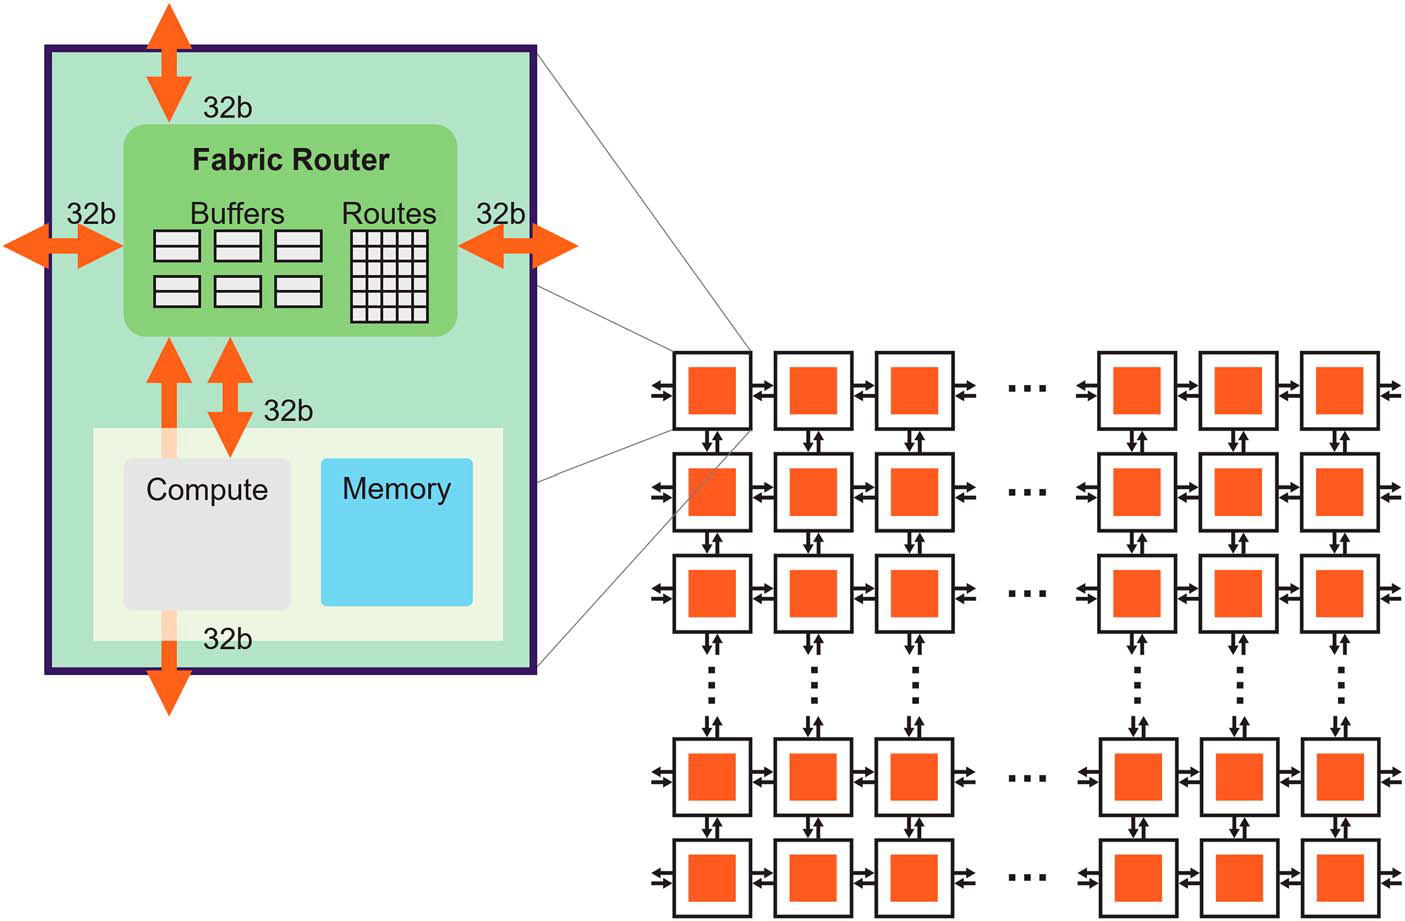
\includegraphics[width=0.5\linewidth]{wse2_pes_router.png}
    \caption{The \ac{wse}-2 has a grid like arrangement of \acp{pe} with a router for each \ac{pe}. The router has a link to the routers of the four neighbouring \acp{pe} as well as to the \ac{ce}. Each of these links has a bidirectional bandwidth of \qty{32}{\bit} per cycle \cite{lie2023cerebras}}
    \label{fig:wse2_pes_router}
\end{figure}

Each \ac{pe} allows to execute certain instructions in parallel with \acp{simd} units. The maximum number of parallel instructions varies between instruction types and \ac{wse} generations. Table \ref{tab:simd_operations} shows the maximum \acp{simd}-width for selected instruction types. As the \ac{wse} was originally designed for \ac{ai} workloads, the \acp{simd} units are optimized for half precision floating point operations, which is are not suitable for \ac{hpc} workloads.

\begin{table}[h]
    \centering
    \caption{Maximum \acp{simd}-width for selected instruction types}
    \label{tab:simd_operations}
    \begin{tabular}{@{}cccc@{}}
        \toprule
        Op code & desciption & \ac{wse}-2 & \ac{wse}-3 \\
        \midrule
        \texttt{@fadds} & 32-bit floating point add & 2 & 4 \\
        \texttt{@fmuls} & 32-bit floating point multiply & 1 & 1 \\
        \texttt{@fmach} & 16-bit floating point multiply-add & 4 & 8 \\
        \texttt{@fmachs} & 16-bit floating point multiply with 32 bit addition & 2 & 4 \\
        \texttt{@fmacs} & 32-bit floating point multiply-add & 1 & 1 \\
        \texttt{@fmovs} & 32-bit floating point move & 2 & 4 \\
        \bottomrule
    \end{tabular}
\end{table}

Custom kernels for the \ac{wse} are written in \ac{csl} which is very low level language based on Zig and extends the language with hardware specific features.
One of its core features is the ability to define \acp{dsd} which define data access patterns including a base memory address, an offset, a stride and a length. They can be used for up to four dimensional tensors. Specifically there are four \ac{dsd} types. \texttt{mem1d\_dsd}, \texttt{mem4d\_dsd}, \texttt{fabin\_dsd} and \texttt{fabout\_dsd}. While \texttt{fabin\_dsd} and \texttt{fabout\_dsd} are used for fabric communication and \texttt{mem1d\_dsd} are used for one dimensional arrays, \texttt{mem4d\_dsd} are somewhat unintuitively used for tensors with two, three or four dimensions. The \ac{wse}-2 has 44 \acp{dsr} per \ac{pe} which are hardware registers used to hold \acp{dsd}. These can be directly used by as operands for instructions. Loading \acp{dsd} into \acp{dsr} is done automatically by the compiler, but can also be done manually and enables the programmer to optimize the code. Communication between \acp{pe} is handled with special fabin- and fabout-\acp{dsd}, describing data that is sent to or received from a neighbouring \ac{pe}.

The routers contain a limited number of input and output queues, small physical buffers for incoming and outgoing data.

\ac{csl} has limited support for concurrency which is enabled by the use of tasks that are activated by events like completion of an asynchronous communication or computation. Due to the single thread of execution, there is no true parallelism within a single \ac{pe}.

optional: ???
- cannot receive and send at same time???
- limitations due to input and output queues? 
